% Options for packages loaded elsewhere
\PassOptionsToPackage{unicode}{hyperref}
\PassOptionsToPackage{hyphens}{url}
%
\documentclass[
]{article}
\usepackage{lmodern}
\usepackage{amssymb,amsmath}
\usepackage{ifxetex,ifluatex}
\ifnum 0\ifxetex 1\fi\ifluatex 1\fi=0 % if pdftex
  \usepackage[T1]{fontenc}
  \usepackage[utf8]{inputenc}
  \usepackage{textcomp} % provide euro and other symbols
\else % if luatex or xetex
  \usepackage{unicode-math}
  \defaultfontfeatures{Scale=MatchLowercase}
  \defaultfontfeatures[\rmfamily]{Ligatures=TeX,Scale=1}
\fi
% Use upquote if available, for straight quotes in verbatim environments
\IfFileExists{upquote.sty}{\usepackage{upquote}}{}
\IfFileExists{microtype.sty}{% use microtype if available
  \usepackage[]{microtype}
  \UseMicrotypeSet[protrusion]{basicmath} % disable protrusion for tt fonts
}{}
\makeatletter
\@ifundefined{KOMAClassName}{% if non-KOMA class
  \IfFileExists{parskip.sty}{%
    \usepackage{parskip}
  }{% else
    \setlength{\parindent}{0pt}
    \setlength{\parskip}{6pt plus 2pt minus 1pt}}
}{% if KOMA class
  \KOMAoptions{parskip=half}}
\makeatother
\usepackage{xcolor}
\IfFileExists{xurl.sty}{\usepackage{xurl}}{} % add URL line breaks if available
\IfFileExists{bookmark.sty}{\usepackage{bookmark}}{\usepackage{hyperref}}
\hypersetup{
  pdftitle={Fish and stroke},
  pdfauthor={Starrfelt},
  hidelinks,
  pdfcreator={LaTeX via pandoc}}
\urlstyle{same} % disable monospaced font for URLs
\usepackage[margin=1in]{geometry}
\usepackage{color}
\usepackage{fancyvrb}
\newcommand{\VerbBar}{|}
\newcommand{\VERB}{\Verb[commandchars=\\\{\}]}
\DefineVerbatimEnvironment{Highlighting}{Verbatim}{commandchars=\\\{\}}
% Add ',fontsize=\small' for more characters per line
\usepackage{framed}
\definecolor{shadecolor}{RGB}{248,248,248}
\newenvironment{Shaded}{\begin{snugshade}}{\end{snugshade}}
\newcommand{\AlertTok}[1]{\textcolor[rgb]{0.94,0.16,0.16}{#1}}
\newcommand{\AnnotationTok}[1]{\textcolor[rgb]{0.56,0.35,0.01}{\textbf{\textit{#1}}}}
\newcommand{\AttributeTok}[1]{\textcolor[rgb]{0.77,0.63,0.00}{#1}}
\newcommand{\BaseNTok}[1]{\textcolor[rgb]{0.00,0.00,0.81}{#1}}
\newcommand{\BuiltInTok}[1]{#1}
\newcommand{\CharTok}[1]{\textcolor[rgb]{0.31,0.60,0.02}{#1}}
\newcommand{\CommentTok}[1]{\textcolor[rgb]{0.56,0.35,0.01}{\textit{#1}}}
\newcommand{\CommentVarTok}[1]{\textcolor[rgb]{0.56,0.35,0.01}{\textbf{\textit{#1}}}}
\newcommand{\ConstantTok}[1]{\textcolor[rgb]{0.00,0.00,0.00}{#1}}
\newcommand{\ControlFlowTok}[1]{\textcolor[rgb]{0.13,0.29,0.53}{\textbf{#1}}}
\newcommand{\DataTypeTok}[1]{\textcolor[rgb]{0.13,0.29,0.53}{#1}}
\newcommand{\DecValTok}[1]{\textcolor[rgb]{0.00,0.00,0.81}{#1}}
\newcommand{\DocumentationTok}[1]{\textcolor[rgb]{0.56,0.35,0.01}{\textbf{\textit{#1}}}}
\newcommand{\ErrorTok}[1]{\textcolor[rgb]{0.64,0.00,0.00}{\textbf{#1}}}
\newcommand{\ExtensionTok}[1]{#1}
\newcommand{\FloatTok}[1]{\textcolor[rgb]{0.00,0.00,0.81}{#1}}
\newcommand{\FunctionTok}[1]{\textcolor[rgb]{0.00,0.00,0.00}{#1}}
\newcommand{\ImportTok}[1]{#1}
\newcommand{\InformationTok}[1]{\textcolor[rgb]{0.56,0.35,0.01}{\textbf{\textit{#1}}}}
\newcommand{\KeywordTok}[1]{\textcolor[rgb]{0.13,0.29,0.53}{\textbf{#1}}}
\newcommand{\NormalTok}[1]{#1}
\newcommand{\OperatorTok}[1]{\textcolor[rgb]{0.81,0.36,0.00}{\textbf{#1}}}
\newcommand{\OtherTok}[1]{\textcolor[rgb]{0.56,0.35,0.01}{#1}}
\newcommand{\PreprocessorTok}[1]{\textcolor[rgb]{0.56,0.35,0.01}{\textit{#1}}}
\newcommand{\RegionMarkerTok}[1]{#1}
\newcommand{\SpecialCharTok}[1]{\textcolor[rgb]{0.00,0.00,0.00}{#1}}
\newcommand{\SpecialStringTok}[1]{\textcolor[rgb]{0.31,0.60,0.02}{#1}}
\newcommand{\StringTok}[1]{\textcolor[rgb]{0.31,0.60,0.02}{#1}}
\newcommand{\VariableTok}[1]{\textcolor[rgb]{0.00,0.00,0.00}{#1}}
\newcommand{\VerbatimStringTok}[1]{\textcolor[rgb]{0.31,0.60,0.02}{#1}}
\newcommand{\WarningTok}[1]{\textcolor[rgb]{0.56,0.35,0.01}{\textbf{\textit{#1}}}}
\usepackage{graphicx,grffile}
\makeatletter
\def\maxwidth{\ifdim\Gin@nat@width>\linewidth\linewidth\else\Gin@nat@width\fi}
\def\maxheight{\ifdim\Gin@nat@height>\textheight\textheight\else\Gin@nat@height\fi}
\makeatother
% Scale images if necessary, so that they will not overflow the page
% margins by default, and it is still possible to overwrite the defaults
% using explicit options in \includegraphics[width, height, ...]{}
\setkeys{Gin}{width=\maxwidth,height=\maxheight,keepaspectratio}
% Set default figure placement to htbp
\makeatletter
\def\fps@figure{htbp}
\makeatother
\setlength{\emergencystretch}{3em} % prevent overfull lines
\providecommand{\tightlist}{%
  \setlength{\itemsep}{0pt}\setlength{\parskip}{0pt}}
\setcounter{secnumdepth}{-\maxdimen} % remove section numbering

\title{Fish and stroke}
\author{Starrfelt}
\date{8 1 2021}

\begin{document}
\maketitle

\hypertarget{modelling-the-health-impacts-of-fish-intake-on-stroke}{%
\subsection{Modelling the health impacts of fish intake on
stroke}\label{modelling-the-health-impacts-of-fish-intake-on-stroke}}

The grading of the scientific evidence deems that there is `probably' a
link between fish consumption and stroke - i.e.~that intake of fish
reduced the probability of stroke. This document is the first attempt to
both show results and code necessary to establish a quantitative link
between the fish intake in Norway and incidence of stroke.

\hypertarget{sources-of-data}{%
\subsection{Sources of data}\label{sources-of-data}}

\hypertarget{dietary-intake}{%
\subsubsection{Dietary intake}\label{dietary-intake}}

Intake is in this example restricted to the adult population, ages 18-70
yrs old. The dietary intake used is from the
\href{https://www.helsedirektoratet.no/rapporter/norkost-3-en-landsomfattende-kostholdsundersokelse-blant-menn-og-kvinner-i-norge-i-alderen-18-70-ar-2010-11/Norkost\%203\%20en\%20landsomfattende\%20kostholdsundersokelse\%20blant\%20menn\%20og\%20kvinner\%20i\%20Norge\%20i\%20alderen-18-70\%20\%C3\%A5r\%202010-11.pdf/_/attachment/inline/b7bafaab-6059-4450-8d76-c3ed9f3eaf3f:be251cd1153cf1ae8e4c46eedddc13b36da3d11d/Norkost\%203\%20en\%20landsomfattende\%20kostholdsundersokelse\%20blant\%20menn\%20og\%20kvinner\%20i\%20Norge\%20i\%20alderen-18-70\%20\%C3\%A5r\%202010-11.pdf}{Norkost
survey} as coded in KBS (Kostberegningssystemet). In practice the
consumption of all types of food and drinks in the lowest level of the
food database (AE18) for 1787 individuals over two days are imported
into R.

Several categorizations of dietary elements related to fish has been
compiled. To get the intake of fish. {[}Perhaps show the grouping used
in this example{]}. In this example I have included all types of `fish'
but removed `other seafood'. Amounts consumed are rescaled for
weight-loss during preparation and content of raw filet pr unit eaten
product. The rescaling and grouping was prepared by Inger-Therese. The
groups are included in the data used in R, the scaling factors are not.

\hypertarget{dose-response-curve-relating-fish-intake-to-stroke-risk.}{%
\subsubsection{Dose-response curve relating fish intake to stroke
risk.}\label{dose-response-curve-relating-fish-intake-to-stroke-risk.}}

\emph{Food groups and risk of coronary heart disease, stroke and heart
failure: A systematic review and dose-response meta-analysis of
prospective studies} by Bechthold et al.~(2017/2019) was used as the
source for the dose response, relating fish intake {[}g/day{]} to
relative risk (RR) of stroke. The dose-response curve was extracted from
Figure 3 using the online version of the
\href{https://automeris.io/WebPlotDigitizer/}{WebPlotDigitizer}.

\hypertarget{incidence-of-stroke-in-norway.}{%
\subsubsection{Incidence of stroke in
Norway.}\label{incidence-of-stroke-in-norway.}}

Data for the incidence of stroke in Norway were gathered from the
Norwegian Cardiovascular Disease Registry (Hjerte- og karregisteret, can
be found \href{http://statistikkbank.fhi.no/hkr/}{here}). Number of
stroke (``Akutt hjerneslag'') diagnoses for males/females in 4 age
groups (0--49, 50--69,70--89,90+) for years 2015--2019 are available.
Here I used the numbers from 2019.

\hypertarget{norwegian-population}{%
\subsubsection{Norwegian population}\label{norwegian-population}}

Oftentimes it is useful to correct dietary intake data for level of
education - it is a strong predictor of the intake of many types of food
and individuals with fewer years of formal education are often less
likely to respond to surveys. Data on both the age-composition of the
adult Norwegian population (SSB:
\href{https://www.ssb.no/statbank/table/07459/}{Table 07459} and age
structured data on level of education (SSB:
\href{https://www.ssb.no/statbank/table/09430/}{Table 09430}) were
gather from \emph{Statistics Norway} (SSB). Data for 2019 were used.

\begin{verbatim}
## Loading required package: Matrix
\end{verbatim}

\begin{verbatim}
## Loading required package: coda
\end{verbatim}

\begin{verbatim}
## Loading required package: ape
\end{verbatim}

\begin{verbatim}
## PACKAGE: org
\end{verbatim}

\begin{verbatim}
## Version 2020.05.25 at 12:01
\end{verbatim}

\begin{verbatim}
## Developed by Richard White, Norwegian Institute of Public Health
\end{verbatim}

\begin{verbatim}
## 
## Attaching package: 'dplyr'
\end{verbatim}

\begin{verbatim}
## The following objects are masked from 'package:stats':
## 
##     filter, lag
\end{verbatim}

\begin{verbatim}
## The following objects are masked from 'package:base':
## 
##     intersect, setdiff, setequal, union
\end{verbatim}

\begin{verbatim}
## `summarise()` regrouping output by 'day' (override with `.groups` argument)
\end{verbatim}

\begin{verbatim}
## `summarise()` ungrouping output (override with `.groups` argument)
\end{verbatim}

\hypertarget{modelling-the-fish-intake}{%
\subsection{Modelling the fish-intake}\label{modelling-the-fish-intake}}

The daily intake of fish calculated was fitted to a generalized
mixed-model using the package MCMCglmm. This package allows for
multivariate approaches and a couple of different models were applied to
the data. The structure of the models could probably be altered and
other applications should perhaps be evaluted, particularly with
random-effects for each sex.

\hypertarget{data-to-be-predicted}{%
\subsubsection{Data to be predicted}\label{data-to-be-predicted}}

The data to be predicted by the model are the categorical (eats fish or
not) and numerical (log amounts fish eaten, if fish is consumed) for the
two days for the 1787 individuals.

\begin{Shaded}
\begin{Highlighting}[]
\KeywordTok{summary}\NormalTok{(cars)}
\end{Highlighting}
\end{Shaded}

\begin{verbatim}
##      speed           dist       
##  Min.   : 4.0   Min.   :  2.00  
##  1st Qu.:12.0   1st Qu.: 26.00  
##  Median :15.0   Median : 36.00  
##  Mean   :15.4   Mean   : 42.98  
##  3rd Qu.:19.0   3rd Qu.: 56.00  
##  Max.   :25.0   Max.   :120.00
\end{verbatim}

\hypertarget{including-plots}{%
\subsection{Including Plots}\label{including-plots}}

You can also embed plots, for example:

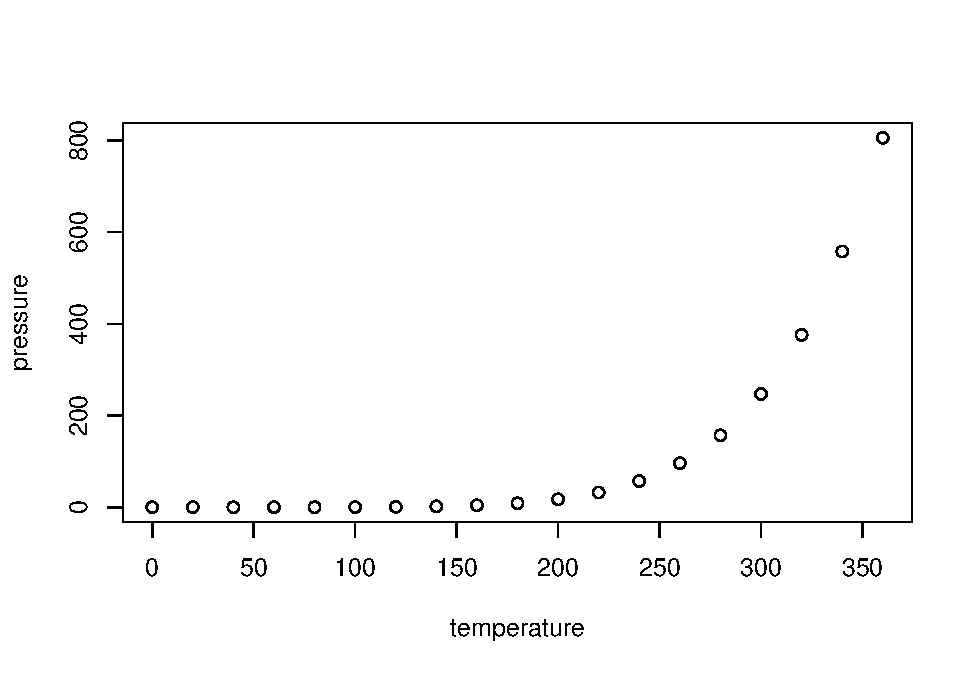
\includegraphics{Fish_n_stroke_2021_files/figure-latex/pressure-1.pdf}

Note that the \texttt{echo\ =\ FALSE} parameter was added to the code
chunk to prevent printing of the R code that generated the plot.

\end{document}
